% ==============================================================================
% GRADUATION THESIS TEMPLATE (ENGLISH VERSION)
% Secondary Technical School and Gymnasium Na Třebešíně
% ==============================================================================

\documentclass[12pt, a4paper, oneside]{article}

% ------------------------------------------------------------------------------
% 1. THESIS METADATA
% ------------------------------------------------------------------------------
\newcommand{\NazevPrace}{Interactive Digital Notebook with Integrated AI Assistant for Education}
\newcommand{\NazevPraceVelkymi}{INTERACTIVE DIGITAL NOTEBOOK WITH INTEGRATED AI ASSISTANT FOR EDUCATION}
\newcommand{\NazevPraceCs}{Interaktivní digitální poznámkový blok s~integrovaným AI asistentem pro výuku}
\newcommand{\Autor}{Kostiantyn Kudinov}
\newcommand{\Vedouci}{Mgr. Jan Souhrada}
\newcommand{\Trida}{4.G}
\newcommand{\SkolniRok}{2026 / 2027}

% ------------------------------------------------------------------------------
% 2. ENCODING, LANGUAGE AND FONTS (Times New Roman 12pt + Arial for headings)
% ------------------------------------------------------------------------------
\usepackage[utf8]{inputenc}
\usepackage[T1]{fontenc}
\usepackage[english]{babel}

% Serif font for body text (Times New Roman / TeX Gyre Termes)
\usepackage{tgtermes}
% Sans-serif font for headings and title page (Arial / TeX Gyre Heros)
\usepackage{tgheros}
% Monospace font for code (TeX Gyre Cursor)
\usepackage{tgcursor}

% Microtypography
\usepackage{microtype}

% ------------------------------------------------------------------------------
% 3. PAGE MARGINS AND LINE SPACING (2.5 cm margins, 1.5 line spacing)
% ------------------------------------------------------------------------------
\usepackage[
    a4paper,
    top=2.5cm,
    bottom=2.5cm,
    left=2.5cm,
    right=2.5cm,
    footskip=1.25cm
]{geometry}

\usepackage{setspace}
\onehalfspacing

\setlength{\parindent}{0pt}
\setlength{\parskip}{6pt}

% ------------------------------------------------------------------------------
% 4. HEADERS, FOOTERS AND PAGE NUMBERING ("- 5 -")
% ------------------------------------------------------------------------------
\usepackage{fancyhdr}

\renewcommand{\thepage}{- \arabic{page} -}

\pagestyle{fancy}
\fancyhf{}
\renewcommand{\headrulewidth}{0pt}
\renewcommand{\footrulewidth}{0pt}
\fancyfoot[C]{\normalfont\fontsize{12pt}{14pt}\selectfont \thepage}

% ------------------------------------------------------------------------------
% 5. HEADING FORMATTING
% ------------------------------------------------------------------------------
\usepackage{titlesec}
\usepackage{etoolbox}

\setcounter{secnumdepth}{4}
\setcounter{tocdepth}{3}

\preto{\section}{\clearpage}

% Heading 1 (\section): 16pt, sans-serif, bold
\titleformat{\section}
    {\normalfont\fontsize{16pt}{20pt}\selectfont\sffamily\bfseries}
    {\thesection}{0.75em}{}
\titlespacing*{\section}{0pt}{0pt}{12pt}

% Heading 2 (\subsection): 14pt, sans-serif, bold + italic
\titleformat{\subsection}
    {\normalfont\fontsize{14pt}{18pt}\selectfont\sffamily\bfseries\itshape}
    {\thesubsection}{0.75em}{}
\titlespacing*{\subsection}{0pt}{12pt}{6pt}

% Heading 3 (\subsubsection): 12pt, sans-serif, bold
\titleformat{\subsubsection}
    {\normalfont\fontsize{12pt}{15pt}\selectfont\sffamily\bfseries}
    {\thesubsubsection}{0.75em}{}
\titlespacing*{\subsubsection}{0pt}{6pt}{6pt}

% Heading 4 (\paragraph)
\titleformat{\paragraph}[hang]
    {\normalfont\fontsize{13pt}{16pt}\selectfont\sffamily\bfseries}
    {\theparagraph}{0.75em}{}
\titlespacing*{\paragraph}{0pt}{6pt}{6pt}

% Non-TOC heading
\newcommand{\nadpismimoobsah}[1]{%
    \vspace{6pt}%
    {\normalfont\fontsize{14pt}{18pt}\selectfont\sffamily\bfseries #1\par}%
    \vspace{2pt}%
}

% ------------------------------------------------------------------------------
% 6. TABLE OF CONTENTS, LIST OF FIGURES AND TABLES FORMATTING
% ------------------------------------------------------------------------------
\makeatletter
\renewcommand{\@pnumwidth}{3.2em}
\renewcommand{\@tocrmarg}{4.0em}

\renewcommand*\l@section[2]{%
  \ifnum \c@tocdepth >\z@
    \addpenalty\@secpenalty
    \addvspace{4pt \@plus\p@}%
    \setlength\@tempdima{1.8em}%
    \begingroup
      \parindent \z@ \rightskip \@pnumwidth
      \parfillskip -\@pnumwidth
      \leavevmode
      \advance\leftskip\@tempdima
      \hskip -\leftskip
      #1\nobreak\leaders\hbox{$\m@th\mkern \@dotsep mu\hbox{.}\mkern \@dotsep mu$}\hfill\nobreak\hb@xt@\@pnumwidth{\hss #2}\par
    \endgroup
  \fi}

\renewcommand*\l@figure[2]{%
  \@dottedtocline{1}{0pt}{5.5em}{Figure~#1}{#2}}

\renewcommand*\l@table[2]{%
  \@dottedtocline{1}{0pt}{5.5em}{Table~#1}{#2}}
\makeatother

% ------------------------------------------------------------------------------
% 7. PACKAGES FOR GRAPHICS, TABLES, MATH, CODE AND LINKS
% ------------------------------------------------------------------------------
\usepackage{graphicx}
\usepackage{float}
\usepackage{url}
\usepackage{booktabs}
\usepackage{array}
\usepackage{tabularx}
\usepackage{amsmath}
\usepackage{amssymb}
\usepackage{enumitem}
\usepackage{xcolor}
\usepackage{listings}

\usepackage[
    font={it},
    labelfont={it},
    labelsep=colon,
    justification=centering
]{caption}

\definecolor{codebg}{rgb}{0.97, 0.97, 0.97}
\definecolor{codeborder}{rgb}{0.85, 0.85, 0.85}
\definecolor{codecomment}{rgb}{0.40, 0.40, 0.40}
\definecolor{codekeyword}{rgb}{0.10, 0.20, 0.70}
\definecolor{codestring}{rgb}{0.15, 0.50, 0.15}

\lstset{
    backgroundcolor=\color{codebg},
    frame=single,
    rulecolor=\color{codeborder},
    basicstyle=\ttfamily\fontsize{9.5pt}{12pt}\selectfont,
    keywordstyle=\color{codekeyword}\bfseries,
    commentstyle=\color{codecomment}\itshape,
    stringstyle=\color{codestring},
    numbers=left,
    numberstyle=\tiny\color{codecomment},
    numbersep=8pt,
    breaklines=true,
    breakatwhitespace=true,
    showstringspaces=false,
    tabsize=2,
    captionpos=b,
    keepspaces=true
}

\usepackage[hypertexnames=false, hidelinks, unicode]{hyperref}


% ==============================================================================
% DOCUMENT BODY
% ==============================================================================
\begin{document}

\pagestyle{empty}

% ------------------------------------------------------------------------------
% PAGE 1: TITLE PAGE
% ------------------------------------------------------------------------------
\begin{center}
    {\sffamily\fontsize{12pt}{15pt}\selectfont Secondary Technical School and Gymnasium Na Třebešíně\par}
    \vspace{6pt}
    {\sffamily\bfseries\fontsize{16pt}{20pt}\selectfont GRADUATION THESIS WITH DEFENSE\par}

    \vspace{1.2cm}
    
\includegraphics[width=5.6cm]{obrazky/logo_skoly.png}

    \vspace{2.2cm}
    {\sffamily\bfseries\fontsize{16pt}{22pt}\selectfont \NazevPraceVelkymi\par}
\end{center}

\vfill

{\sffamily\fontsize{10pt}{14pt}\selectfont
\begin{tabular}{@{}p{3.5cm}l@{}}
    Author:     & \Autor \\[6pt]
    Supervisor: & \Vedouci \\[6pt]
    Class:      & \Trida \\[6pt]
    School Year:& \SkolniRok \\
\end{tabular}
}

\vspace{0.5cm}
\clearpage

% ------------------------------------------------------------------------------
% PAGE 2: OFFICIAL ASSIGNMENT (SCANNED DOCUMENT)
% ------------------------------------------------------------------------------
\noindent
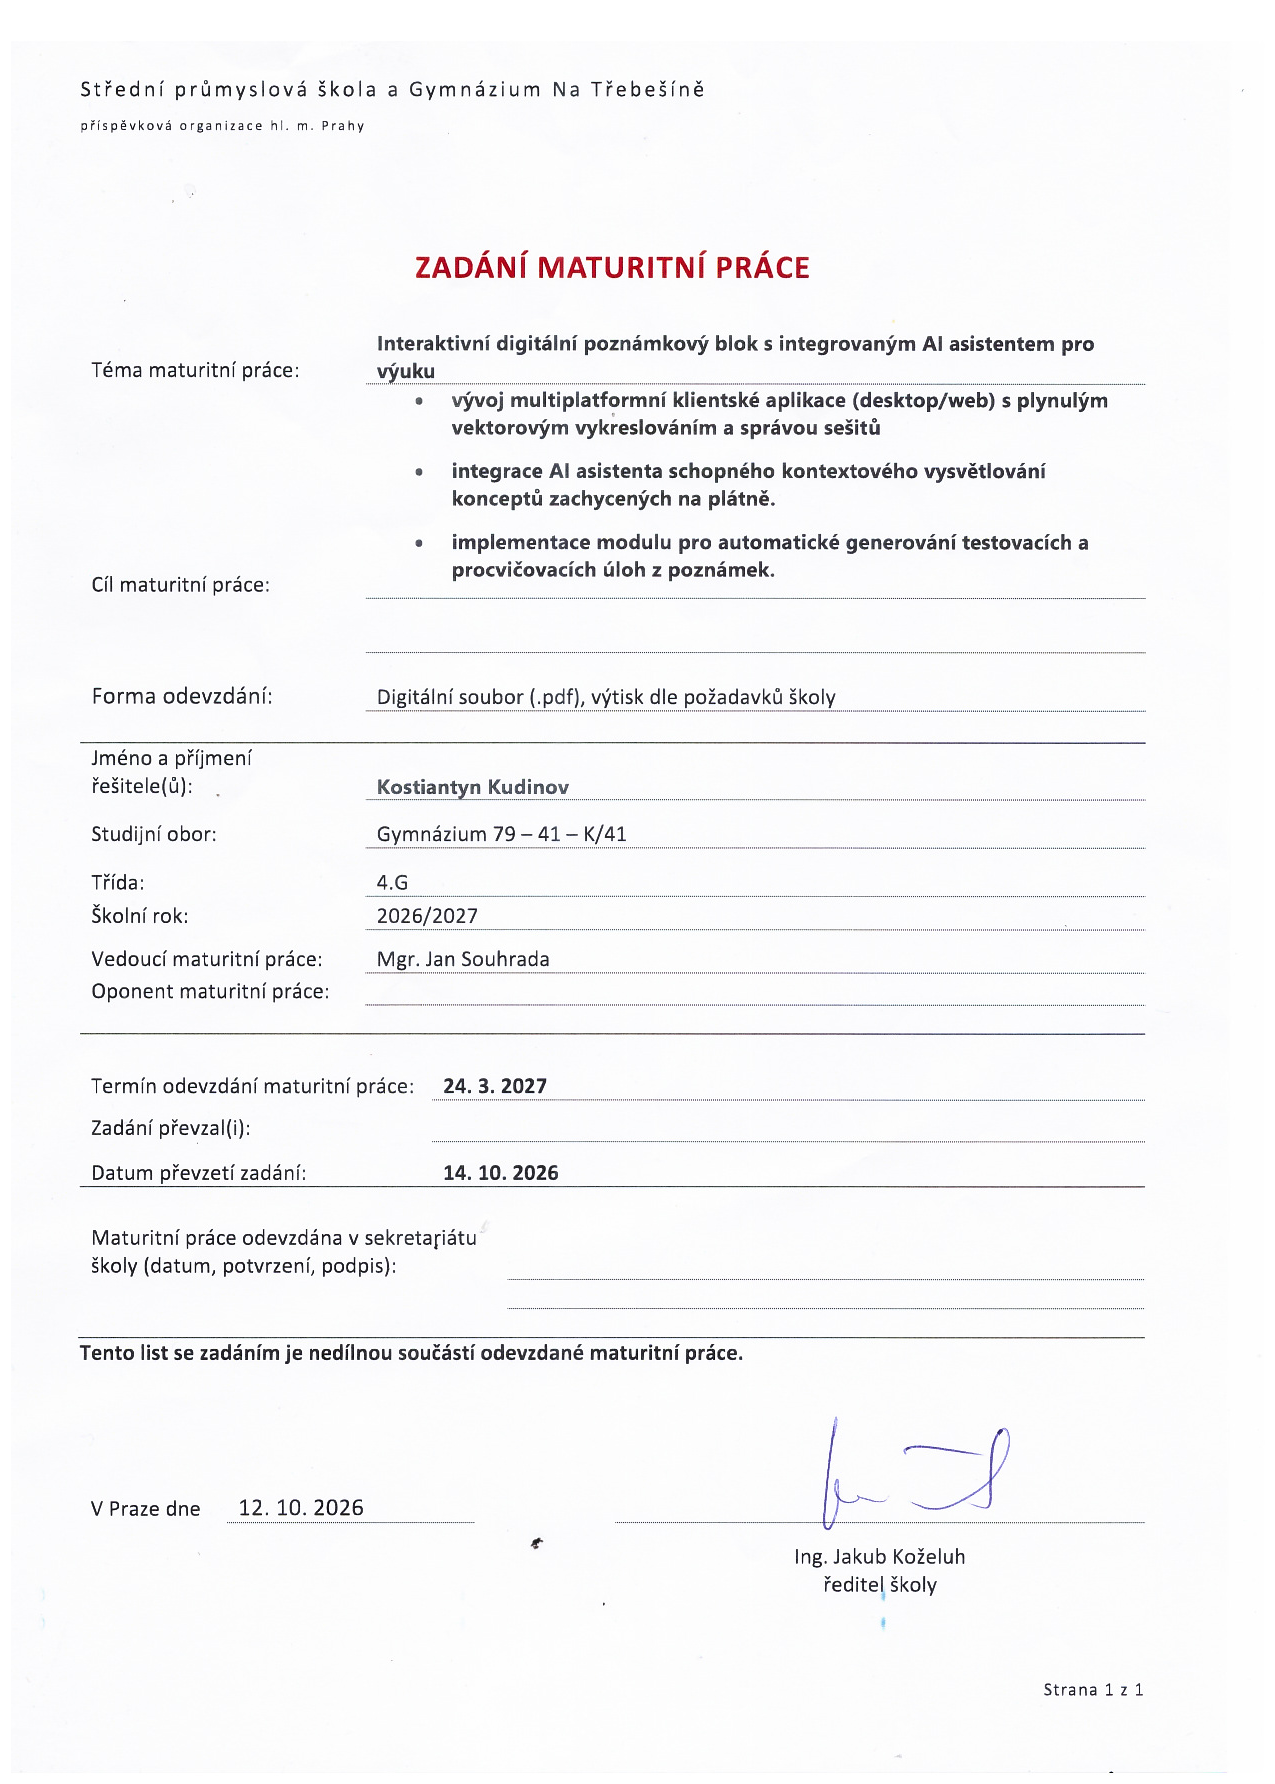
\includegraphics[width=\textwidth]{obrazky/zadani.png}

\clearpage

% ------------------------------------------------------------------------------
% PAGE 3: DECLARATION OF AUTHENTICITY
% ------------------------------------------------------------------------------
\vspace*{7.5cm}

\nadpismimoobsah{Declaration of Authenticity}

I hereby declare that I have completed this graduation thesis on the topic of \textbf{\NazevPrace} independently, using the professional literature and sources listed in the attached list of references.

\vspace{1.2cm}
In Prague, Date: \makebox[4cm]{\dotfill}

\vspace{1.8cm}
\makebox[6cm]{\dotfill} \\
\textit{Author's signature}

\clearpage

% ------------------------------------------------------------------------------
% PAGE 4: ACKNOWLEDGEMENTS
% ------------------------------------------------------------------------------
\vspace*{6.5cm}

\nadpismimoobsah{Acknowledgements}

I would like to express my sincere gratitude to my graduation thesis supervisor, \textbf{\Vedouci}, for his professional guidance, valuable feedback, insightful advice, and the time dedicated to consultations throughout the preparation of this thesis.

\clearpage

% ==============================================================================
% PAGE 5 ONWARDS: NUMBERING IN FOOTER ("- 5 -")
% ==============================================================================
\pagestyle{fancy}
\setcounter{page}{5}

% ------------------------------------------------------------------------------
% PAGE 5: ANNOTATION (ENGLISH)
% ------------------------------------------------------------------------------
\nadpismimoobsah{Thesis Title:}
\NazevPrace

\nadpismimoobsah{Author:}
\Autor

\nadpismimoobsah{Supervisor:}
\Vedouci

\nadpismimoobsah{Abstract}
The objective of this graduation thesis is to design, implement, and evaluate a lightweight, cross-platform digital notebook and virtual whiteboard application with an integrated artificial intelligence assistant for educational workflows and self-directed study. The application combines the flexibility of an infinite zoomable canvas (ZUI) for mind mapping and brainstorming with a structured, paginated ISO 216 A4 notebook capable of importing and annotating PDF documents. The desktop client is engineered using Tauri~v2, Rust, and React, utilizing immediate-mode HTML5 Canvas rendering for responsive, low-latency drawing. Designed with a Local-First architecture, user data is stored primarily on the local disk in a portable format, ensuring offline privacy, data ownership, and instant access. Furthermore, an interactive multimodal AI tutor is integrated to provide step-by-step explanations of handwritten calculations and generate context-aware practice exercises.

\nadpismimoobsah{Keywords}
digital notebook, virtual whiteboard, Tauri v2, Rust, React, TypeScript, HTML5 Canvas, Local-First, offline-first, PDF annotation, artificial intelligence, multimodal AI

\clearpage

% ------------------------------------------------------------------------------
% PAGE 6: ANNOTATION (CZECH SUMMARY)
% ------------------------------------------------------------------------------
\nadpismimoobsah{Název práce:}
\NazevPraceCs

\nadpismimoobsah{Autor:}
\Autor

\nadpismimoobsah{Vedoucí práce:}
\Vedouci

\nadpismimoobsah{Abstrakt}
Cílem této maturitní práce je navrhnout, implementovat a~otestovat odlehčený, multiplatformní digitální poznámkový blok a~virtuální tabuli s~integrovaným asistentem na bázi umělé inteligence pro podporu výuky a~samostatného studia. Aplikace kombinuje výhody neomezené plochy (ZUI) pro volné myšlenkové mapy se stránkovaným sešitem formátu A4 a~možností importu i~anotování dokumentů PDF. Klientská vrstva je postavena na frameworku Tauri~v2, jazyce Rust a~knihovně React s~využitím HTML5 Canvasu pro plynulé vykreslování s~minimální latencí. Díky architektuře Local-First jsou veškeré poznámky ukládány primárně lokálně na disk v~přenosném formátu bez nutnosti registrace. Součástí aplikace je také integrovaný multimodální AI asistent pro kontextové vysvětlování ručně psané látky a~tvorbu procvičovacích úloh.

\nadpismimoobsah{Klíčová slova}
digitální poznámkový blok, virtuální tabule, Tauri v2, Rust, React, TypeScript, HTML5 Canvas, Local-First, offline-first, anotace PDF, umělá inteligence, multimodální AI

\clearpage

% ------------------------------------------------------------------------------
% PAGE 7: TABLE OF CONTENTS
% ------------------------------------------------------------------------------
\nadpismimoobsah{Contents}
\makeatletter
\@starttoc{toc}
\makeatother

\clearpage

% ==============================================================================
% 1 INTRODUCTION
% ==============================================================================
\section{Introduction}
\label{sec:uvod}

When studying technical disciplines and computer science, conventional word processors such as Microsoft Word or Google Docs quickly prove insufficient. Writing mathematical formulas, drawing schematics, and sketching algorithms within linear text editors is cumbersome and inefficient. A much more natural approach is writing and drawing freehand on a digital canvas or annotating lecture slides directly in PDF format.

However, existing software solutions for digital note-taking suffer from distinct drawbacks. Most tools lack native Linux support, and the remainder are largely built upon the Electron framework, which incurs substantial RAM overhead and noticeable input latency due to the embedded Chromium engine. Furthermore, many commercial products require mandatory online user accounts and force cloud storage. Consequently, users lose direct control over their files and cannot access their study materials without an active internet connection.

Virtually the only widespread application that circumvents these issues and runs natively on Linux is Xournal++. In several respects, however, it lags behind modern digital notebooks: it lacks an infinite canvas mode, cannot run in a web browser, and relies on a traditional desktop user interface that buries features inside complex menus and small toolbar buttons, making touch and stylus interaction cumbersome.

This thesis focuses on developing a lightweight digital notebook that unites the clean user experience of modern applications with the fast, efficient Local-First philosophy of Xournal++. The application functions as a desktop program for Linux and Windows, while also supporting execution directly in a web browser and on Android mobile devices. The application combines an infinite canvas for open-ended mind mapping with a structured A4-paginated notebook. Notes are stored primarily locally on disk in a portable format. In addition, the application integrates an intuitive AI assistant designed to help students understand challenging material or generate relevant practice exercises directly from their notes.

% ------------------------------------------------------------------------------
% 1.1 OBJECTIVES OF THE THESIS
% ------------------------------------------------------------------------------
\subsection{Objectives of the Thesis}
\label{sec:cile_prace}

\begin{enumerate}
    \item Develop a cross-platform digital notebook application using the Tauri~v2 framework, Rust, and React.
    \item Implement an interactive canvas offering a choice between an infinite workspace and an A4-paginated notebook, including support for importing and annotating PDF documents.
    \item Ensure Local-First file persistence on disk in a custom portable format, with optional cloud synchronization capabilities.
    \item Integrate an interactive AI assistant to generate explanations and practice questions based on the context of the notebook.
\end{enumerate}


% ==============================================================================
% 2 THEORETICAL BACKGROUND
% ==============================================================================
\section{Theoretical Background}
\label{sec:teoreticka_cast}

This theoretical chapter examines the key concepts upon which the application is designed. It covers human-computer interaction (HCI) in digital note-taking environments, the mathematical principles of 2D computer graphics and coordinate transformations, the fundamentals of the Local-First architecture, and an evaluation of the chosen software stack.

% ------------------------------------------------------------------------------
% 2.1 DIGITAL WORKSPACES AND USER INTERFACES
% ------------------------------------------------------------------------------
\subsection{Digital Workspaces and User Interfaces}
\label{sec:teorie_zui}

In note-taking software, two contrasting approaches to workspace organization predominate: boundless spatial canvases and discrete paginated documents.

\subsubsection{Concept of the Infinite Canvas (ZUI)}
The infinite canvas concept originates from the \textit{Zoomable User Interface} (ZUI) paradigm, whose theoretical foundations were laid by Perlin and Fox in 1993 and further developed by Bederson and Hollan~\cite{bederson1994pad}. In a ZUI, the workspace is not constrained by physical window boundaries or paper margins; the scene exists within a continuous two-dimensional Euclidean plane $\mathbb{R}^2$. Users navigate this space using two fundamental degrees of freedom:
\begin{itemize}
    \item \textbf{Panning:} Translating the virtual camera along the $x$ and $y$ axes to explore extensive diagrams and mind maps.
    \item \textbf{Zooming:} Smoothly adjusting the magnification factor to inspect information across different levels of semantic detail---from a bird's-eye overview of an entire course down to fine handwritten mathematical derivations.
\end{itemize}

The primary advantage of a ZUI is eliminating cognitive friction during brainstorming, as users are never required to guess or allocate page budgets in advance.

\subsubsection{Paginated Notebooks and the ISO 216 Standard}
While a ZUI excels during unstructured planning, systematic study and lecture preparation require predictable exporting and printing. Educational materials, exams, and worksheets are grounded in the international standard ISO~216~\cite{iso216}, which defines the metric A-series format. The base format A0 has an area of exactly $1\text{ m}^2$ and an aspect ratio of $1 : \sqrt{2}$, ensuring that folding a sheet in half preserves the exact proportion (the Lichtenberg ratio). The ubiquitous A4 format ($210 \times 297\text{ mm}$) serves as an ideal baseline for digital notebooks: it provides familiar visual boundaries, simplifies importing and annotating lecture slides, and enables direct printing without unintended cropping.

% ==============================================================================
% 3 PRACTICAL PART
% ==============================================================================
\section{Practical Part}
\label{sec:prakticka_cast}

\textit{(This chapter will be elaborated during project implementation.)}


% ==============================================================================
% 4 CONCLUSION
% ==============================================================================
\section{Conclusion}
\label{sec:zaver}

\textit{(To be completed upon final project implementation and goal evaluation.)}


% ==============================================================================
% 5 REFERENCES (ISO 690)
% ==============================================================================
\section{References}
\label{sec:zdroje}

\begingroup
\sloppy
\renewcommand{\section}[2]{}%
\begin{thebibliography}{99}

    \bibitem{bederson1994pad}
    BEDERSON, Benjamin B. and James D. HOLLAN. Pad++: A~Zooming Graphical Interface for Exploring Alternate Interface Physics. In: \textit{Proceedings of the 7th Annual ACM Symposium on User Interface Software and Technology (UIST '94)} [online]. New York: ACM, 1994, pp.~17--26 [accessed 2026-11-04]. ISBN 0-89791-657-3. Available at: \url{https://doi.org/10.1145/192426.192435}

    \bibitem{iso216}
    INTERNATIONAL ORGANIZATION FOR STANDARDIZATION. \textit{ISO 216:2007 Writing paper and certain classes of printed matter -- Trimmed sizes} [online]. Geneva: ISO, 2007 [accessed 2026-11-04]. Available at: \url{https://www.iso.org/standard/36631.html}

\end{thebibliography}
\endgroup


% ==============================================================================
% 6 APPENDICES
% ==============================================================================
\clearpage
\section*{Appendices}
\addcontentsline{toc}{section}{Appendices}

\textit{(Appendices will be provided upon thesis submission.)}

\end{document}
